\subsection{Architettura}
L'architettura del Sistema Operativo Android è suddivisa in 4 livelli principali \cite{androiden}: 
\begin{itemize}
    \item Linux Kernel
    \item Libraries
    \item Application Framework
    \item Applications
\end{itemize}

Come visto nelle sezioni precedenti, la base di Android è il \textit{kernel Linux}, un insieme di software (detti \textit{driver}) che servono per interfacciarsi con l'hardware, permettono quindi la gestione (a basso libello) di elementi come: schermo, fotocamera, memoria, connettività, ecc. 

Per accedere a tali funzionalità non lo si fa in modo diretto, ma sono presenti delle librerie, scritte in C, che operano come un intermediario (\textit{astrazione} ad un livello superiore). È proprio questo lo scopo del livello \textit{Libraries}. Per semplificarne ancora di più l'utilizzo al programmatore, a queste librerie si accede tramite un \textit{API} Java, il linguaggio principale utilizzato per scrivere applicazioni Android. Perciò, nel sistema è integrata una speciale \textit{Java Virtual Machine} (JVM) chiamata \textit{Dalvik}, creata da Google per poter funzionare anche su dispositivi dotati di risorse molto limitate. \textit{Dalvik}, a differenza della JVM di \textit{SUN} (ora parte di Oracle Corporation) e simili, esegue archivi di tipo \textit{.dex}, un formato che risulta più compatto ed ottimizzato a differenza del \textit{.class}. Non si ha accesso a tutte le API messe a disposizione da JavaSE o JavaME, ma è presente un loro sottoinsieme chiamato \textit{Core Libraries}.\\
Questi due elementi fanno parte di un sottoinsieme del livello \textit{Libraries} chiamato \textit{Android Runtime}.

% potrei aggiungere una descrizione del ciclo di vita di un app
La parte più importante del livello \textit{Application Framework} è l'\textit{Activity Manager}, un particolare componente che si occupa della gestione del ciclo di vita delle applicazioni. È importante notare che ogni applicazione Android viene eseguita da un'istanza della Dalvik VM all'interno di una \textit{sandbox}: un particolare spazio isolato dal resto del sistema in modo da aggiungere uno strato di sicurezza in più.

Infine, nell'ultimo livello risiedono le varie applicazioni installate nel sistema.

\subsubsection{Dalvik VM e ART}
Come scritto in precedenza, il linguaggio con cui vengono programmate le Applicazioni Android è Java e quindi si è introdotta la Dalvik VM all'interno del sistema. Questa non utilizza lo standard \textit{bytecode} delle normali JVM ma ne ha uno proprio ideato apposta per le esigenze di Android. Questo è un sistema \textit{multitasking} e permette alle applicazioni di essere \textit{multithreaded} (di utilizzare più processori), in aggiunta, ogni app viene eseguita in una propria sandbox con la propria istanza della Dalvik VM. Sono proprio questi motivi che impongono alla Dalvik VM di essere leggera e di dover avere un basso \textit{overhead}.

Questa VM compila i programmi Java quasi come tutte le altre, ha solo una differenza: invece di dare come risultato file \textit{.class}, che poi verranno compressi in archivi \textit{.jar}, crea file in formato \textit{.dex} che saranno poi raggruppati in archivi \textit{.apk} (il formato standard della applicazioni Android). Il formato \textit{.dex} per risultare leggero contiene solo \textit{informazioni uniche} \cite{androiden}: se, per esempio, diversi file hanno in comune alcune stringhe, queste appariranno in un solo file .dex, mentre negli altri sarà presente il loro riferimento (\textit{puntatore}). Lo stesso meccanismo è applicato per costanti, oggetti e funzioni.

Dalla versione \textit{5.0 Lollipop} di Android la Dalvik VM è stata rimpiazzata con l'\textit{Android Runtime} (ART) \cite{androiden}. La sostanziale differenza tra le due è quando effettuano la conversione da \textit{bytecode} a \textit{codice macchina}: la vecchia Dalvik utilizza una compilazione \textit{Just In Time} (JIT) \cite{androidwikipedia}, durante l'esecuzione dell'applicazione effettua la conversione quando è necessario; ART usa una compilazione \textit{ahead-of-time} (AOT) \cite{androidwikipedia} cioè tutto il bytecode viene convertito durante la fase di installazione dell'applicazione. Ciò garantisce la necessità di impiegare meno risorse per l'esecuzione delle applicazioni e assicura una maggior fluidità e responsività del sistema. 

\begin{figure}[H]
  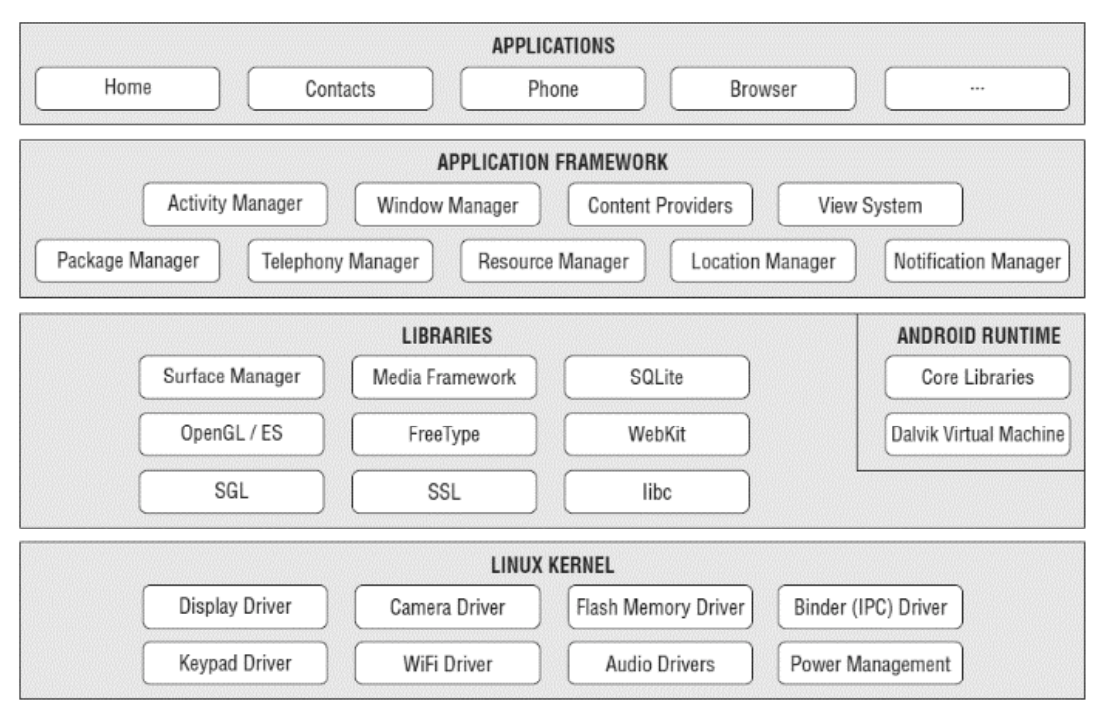
\includegraphics[scale=0.62]{android/imgs/os_architecture.png}
  \caption{Architettura di Android}
  Questo è uno schema riassuntivo dell'architettura di Android prima della versione \textit{Lollipop 5.0}
\end{figure}